\documentclass[UTF8]{ctexart}

% 导入包
\usepackage{listings}
\usepackage{xcolor}
\usepackage{graphicx}

\usepackage[a4paper]{geometry}
\geometry{left=1.91cm, right=1.91cm, top=2.54cm, bottom=2.54cm,}
\setlength{\footskip}{3cm}

% 文档信息
\title{UXLock课程设计报告}
\author{Functioner@sjtu.edu.cn}
\date{2022.12.15}

\lstset{
 columns=fixed,       
%  numbers=left,                                        % 在左侧显示行号
 numberstyle=\tiny\color{gray},                       % 设定行号格式
 frame=none,                                          % 不显示背景边框
 backgroundcolor=\color[RGB]{245,245,244},            % 设定背景颜色
 keywordstyle=\color[RGB]{40,40,255},                 % 设定关键字颜色
 numberstyle=\footnotesize\color{darkgray},           
 commentstyle=\it\color[RGB]{0,96,96},                % 设置代码注释的格式
 stringstyle=\rmfamily\slshape\color[RGB]{128,0,0},   % 设置字符串格式
 showstringspaces=false,                              % 不显示字符串中的空格
 language=c++,                                        % 设置语言
}

\begin{document}

% 放置标题
\maketitle

% 1
\section{同步原语}

% 1.1
\subsection{临界区}
\textbf{定义} 临界区指的是一个访问共用资源(例如:共用设备或是共用存储器)的程序片段,而这些共用资源又无法同时被多个线程访问的特性;当有线程进入临界区段时,其他线程或是进程必须等待。

% 1.2
\subsection{关键路径}
\textbf{定义} 关键路径通常是指同步逻辑电路中,组合逻辑时延最大的路径。
在同步锁问题中,由于临界区的访问权只在“当前持有锁的线程”上,而“传递锁的所有权”也是“临界区的一部分代码”,只不过这部分代码一般不在用户态的代码中。

% 2
\section{基本锁策略}

% 2.1
\subsection{TAS 锁}
最朴素的自旋锁策略,调用者不会进入睡眠状态,如果锁已经被别的线程持有,调用者就在 while 循环中一直使用原子操作直到操作成功。

\textbf{优点} 实现简单,代码量少,能够直观地表现进入区、临界区、退出区。

\textbf{缺点} 只适用于临界区较短、线程数较少的场景,否则正在执行临界区的线程会多次被同一个核心的其他线程的自旋而抢占;无法保证公平性,锁的传递完全凭线程所在CPU的性能,性能较差的核心很容易饥饿。

\begin{lstlisting}
do {
    while(Test_And_Set(&lock));
    /* Critical section */
    lock = False;
} while(True)
\end{lstlisting}

% 2.2
\subsection{CLH 锁}

\textbf{定义} CLH(Craig, Landin, Hagersten三位作者的缩写)队列锁是一种基于链表的可扩展、高性能、公平的自旋锁。维护一个反向队列,申请线程通过原子操作进入队列,之后不断轮询前驱的状态,如果发现前驱释放了锁就结束自旋。

% 2.2.1
\subsubsection{数据结构}
\begin{itemize}
    \item 链表
    \item 尾节点指针
\end{itemize}

\begin{lstlisting}
struct QNode {
    bool locked;
    QNode *prev;
};

QNode *tail;
\end{lstlisting}

% 2.2.2
\subsubsection{线程拿锁}

将自己的 locked 字段设为 true 后入队,之后在前驱节点的 locked 字段上自旋,直到前驱节点状态改变。

\begin{lstlisting}
void lock(QNode *node) {
    node->locked = true; // Set lock field
    node->prev = getAndSet(&tail, node); // Enqueue
    if (node->prev) {
        while (node->prev->locked){
            // Spin until the previous node release
        }
        // May need to free the previous node's memory
    }
    // Enter critical section
}
\end{lstlisting}

% 2.2.3
\subsubsection{线程放锁}

将自己的 locked 字段设为 false 后,直接返回,节点的引用将留在全局 tail 指针或后继节点的 prev 字段中。

\begin{lstlisting}
void unlock(QNode *node) {
    node->locked = false; // Unset lock field
}
\end{lstlisting}

% 2.2.4
\subsubsection{分析}

\begin{itemize}
    \item 由于节点需要在前驱节点自旋,因此在锁的数据结构初始化时,需要添加一个 locked 字段永远为 true 的哨兵节点;
    \item 线程拿锁时申请内存构造一个节点,在结束自旋、进入临界区前,需要将前驱节点的内存释放,在放锁时只需要放弃节点的所有权而不需要释放其内存。只有这样才能满足内存平衡,使得算法在代码层面自洽;
    \item 因此,队列中永远存在一个哨兵节点,这个哨兵节点要么是最开始初始化的那个,要么是最后一个获取锁的线程的节点,它必须留下直到下一个线程到来将它释放;
    \item 节点结构体的 prev 字段实际上可以不需要;
\end{itemize}

\textbf{优点} 由于是排队锁,完全按照先来后到的原则传递锁的所有权,非常公平,不可能出现饥饿;在 SMP 系统结构下非常有效。

\textbf{缺点} 在非对称架构下,如果前驱节点在较远的核心上,则轮循获取其字段的开销较高,因此不适用于 NUMA 结构。

% 2.3
\subsection{MCS 锁}

\textbf{定义} MCS 与 CLH 非常相似,与 CLH 是在前趋节点的 locked 字段上自旋等待的规则不同,MCS 的节点是在自己的 locked 字段上自旋等待。

% 2.3.1
\subsubsection{数据结构}
\begin{itemize}
    \item 链表
    \item 尾节点指针
\end{itemize}

\begin{lstlisting}
struct QNode {
    bool locked;
    QNode *next;
};

QNode *tail;
\end{lstlisting}

% 2.3.2
\subsubsection{线程拿锁}

将自己的 locked 字段设为 true 后入队,之后在自己的 locked 字段上自旋,直到状态被前驱节点改变。

\begin{lstlisting}
void lock(QNode *node) {
    node->locked = true; // Set lock field
    QNode *prev = getAndSet(&tail, node); // Enqueue
    if (prev) {
        prev->next = node;
        while (node->locked){
            // Spin until the field is changed by the previous thread
        }
    }
    // Enter critical section
}
\end{lstlisting}

% 2.3.3
\subsubsection{线程放锁}

如果存在后继节点,那么将后继节点解除自旋。

\begin{lstlisting}
void unlock(QNode *node) {
    if (node->next) {
        node->next->locked = false;
    }
    // May need to free the node's memory
}
\end{lstlisting}

% 2.3.4
\subsubsection{分析}

\textbf{优点} 具备 CLH 锁的所有优点,而且在等待时不需要跨CPU访问其他节点的字段,解决了 CLH 锁在 NUMA 架构中表现出的问题。

\textbf{缺点} 由于通过先来后到原则保证了绝对公平,如果存在一些较晚获取锁但是临界区很短的线程,那么这些线程的等待时间会远远超过其临界区的执行时间,因此 MCS 策略下所有线程的平均时延较高。这同样也是 CLH 锁的缺点。

% 3
\section{设计需求}

% 3.1
\subsection{Mutex 与等待策略}

Mutex 称为互斥锁,Linux 中的 pthread 是一种非常经典的互斥锁的实现。它的底层逻辑是 spin-then-park,线程拿锁后会自旋一段时间,如果这段时间内没有成功获取到锁,就会使用 futex API 放弃处理机资源进入睡眠状态;其他线程放锁后,如果没有活跃线程便会调用 futex API 将其唤醒;

Mutex 本质上与 TAS 锁是相同的,只是等待策略换成了spin-then-park,依然无法保证公平性。

% 3.2
\subsection{MCS 相关}

MCS 如果使用只自旋的等待策略,那么线程数量一旦过多,就会陷入与 TAS 同样的困境,大量处于等待状态的线程会与正在执行临界区的线程抢占 CPU,给关键路径带来大量时延,并且也会消耗大量能源;

MCS 如果使用 spin-then-park 的等待策略,那么在队列后面的线程会全部进入睡眠状态,如果不考虑自我唤醒,那么当锁传递到后面时,所有线程都需要经历一次唤醒,而唤醒是系统调用,也会给关键路径带来没有必要的开销。而如果向普通的 MCS 引入自我唤醒,最终表现出来的效果也是随机的,无法适应场景。

% 3.3
\subsection{公平的代价}

大量短临界区线程与长临界区线程共存时,短临界区线程往往无法承担等待时间很长的代价;虽然 Mutex 无法保证公平性,但是存在很多后拿锁的短线程能提前获得锁,减少了周转时间,因此总体能表现出较好的平均时延和吞吐量;但是由于不公平导致了饥饿,最不幸运的那个线程往往等待了非常久的时间,因此尾时延表限较差;

对于 MCS 来说,由于维护了公平性,能够保证所有线程都能在一定时间内获取到锁,因此将尾时延降到最低,但是大量短线程的等待时间远远大于其临界区时间,因此平均时延表现不好。

% 3.4
\subsection{设计目标}

\textbf{主要矛盾} 锁的调度中,关于等待策略存在一个矛盾,即功耗(Power Consumption)和效率(Energy Efficiency)之间的矛盾,一方面,忙等有利于在锁传到时立即开始执行临界区,而睡眠需要先进行唤醒因而给关键路径引起不必要的开销;另一方面,忙等可能造成线程争抢处理机资源,也会引起功耗较高,而睡眠没有这个问题。

\textbf{关于设计} 对于一个特定场景的锁调度问题,往往需要综合自旋与睡眠的等待策略,设计一个比基本策略稍微复杂一些的调度策略,使吞吐量与能量利用率都得到一定程度的提高。


% 4
\section{进阶策略}

% 4.1
\subsection{Malthusian}

\begin{figure}[ht]
\centering
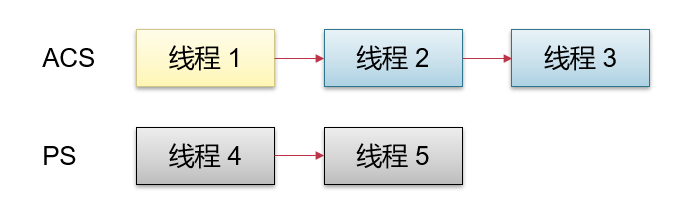
\includegraphics[scale=0.5]{images/img1.png}
\end{figure}

% 4.1.1
\subsubsection{概述}

维护两个队列,一个为活跃队列(Active Circulating Set),一个为阻塞队列(Passive Set),活跃队列为一个类似 MCS 的队列,通过放锁时对两个对列重新排序,使部分线程进入阻塞队列中睡眠,另一部分线程留在活跃队列中能够快速获取锁,既保证锁被充分竞争,又能合理控制竞争激烈程度,长期来看也是公平的。

% 4.1.2
\subsubsection{具体策略}

\begin{enumerate}
    \item 线程拿锁时,简单使用 MCS 的方式进入活跃队列;
    \item 线程放锁时,如果当前线程与活跃队列队尾还有线程,则将一个后继线程放入阻塞队列,否则从阻塞队列中唤醒一个线程到活跃队列中,然后将锁传递给后继的线程;
    \item 为保证长期公平性,线程长时间进入阻塞队列后会被唤醒进入活跃队列;
\end{enumerate}

% 4.1.3
\subsubsection{优点}
\begin{enumerate}
    \item 维持了一定数量的活跃线程,使锁能够被充分竞争,将多余的线程放置到阻塞队列中,不至于让正在执行临界区的线程反复被打断,一定程度上提高了吞吐量;
    \item 通过定期地重排锁队列,在活跃队列和阻塞队列之间转移线程,提供长期的公平性,节省了共享资源,还可以减少抖动效应和性能下降;
\end{enumerate}

% 4.1.4
\subsubsection{缺点}

需要在放锁后维护两个队列,而维护队列的逻辑一旦复杂,就会给关键路径额外开销。

% 4.2
\subsection{Mutexee}

% 4.2.1
\subsubsection{实验与推论}

\begin{enumerate}
    \item 两种等待策略

    首先使用 java.util.concurrent.CopyOnWriteArrayList 为临界区数据结构,来测试 Mutex 与 Spinlock 的吞吐量与功耗,最后得到 Mutex 节省 50\% 的能耗而 Spinlock 的吞吐量是 Mutex 的两倍的结果。

    \begin{figure}[ht]
        \centering
        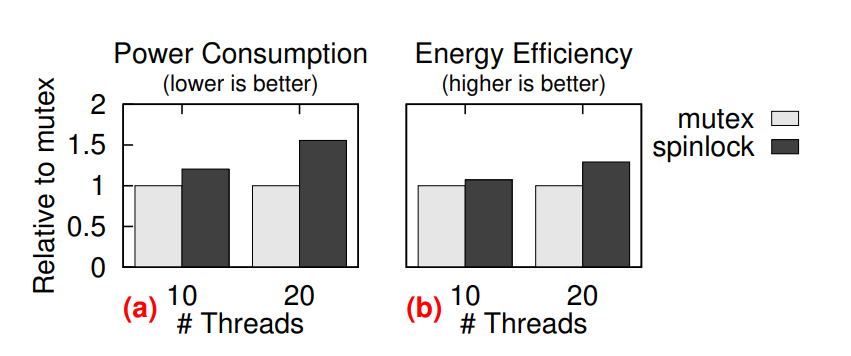
\includegraphics[scale=0.4]{images/img2.png}
    \end{figure}

    可以得到以下结论:

    \begin{itemize}
        \item 自旋会大大增加能耗,在忙等时,底层硬件上下文保持活动状态。例如,在 Intel 的机器上,减少忙等的功耗实际上是不可实现的;
        \item 睡眠会节省能量但因唤醒操作导致低吞吐量,能量利用率较低;
        \item 当一个线程处于活跃状态,不管它执行的是什么类型的工作都会消耗能量。如果它在等待时是阻塞态,那么这部分能量可以节省;
        \item Pthread 调用 futex 系统调用来实现睡眠,然而在大多数现实的场景中,频繁的 futex 调用开销 (唤醒一个正在沉睡的线程至少需要 7000 个周期) 抵消了睡眠所带来的能源收益,从而导致更糟糕的能源效率;
    \end{itemize}

    \item 两个交替线程

    尝试了一种极端的情况,即只有两个线程通过忙等待进行通信,而其余线程都在睡觉。每个活动线程都有一个忙碌等待重复的“配额”T,在此之后,它会唤醒另一个线程来轮流执行。

    \begin{figure}[ht]
        \centering
        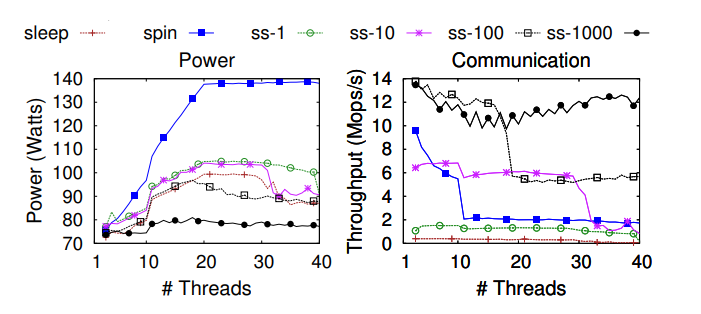
\includegraphics[scale=0.5]{images/img4.png}
    \end{figure}

    可以得到,执行越不公平(例如,对于大T),效率就越好。首先,较大的T值导致较低的功率,因为睡眠和唤醒调用变得不频繁,因此睡眠线程休眠时间较长。其次,自旋的竞争较小,因为只有两个线程试图获取 cache line。因此,锁传递多发生(99.9\%)在自旋中,延迟非常低,导致高吞吐量。

\end{enumerate}

% 4.2.2
\subsubsection{需要解决的互斥锁的问题}

\begin{itemize}
    \item 一些线程的临界区时间可能比 futex 阻塞与唤醒的系统调用时间短;
    \item Mutex 在线程放锁后会如果没有其它线程拿锁,会立即唤醒睡眠的线程,但如果有其它线程在被唤醒的线程能够执行前拿锁,被唤醒的线程可能迟迟拿不到锁又进入到睡眠状态,本次唤醒就无效了;
\end{itemize}

% 4.2.3
\subsubsection{具体策略}

\begin{enumerate}
    \item 相比普通互斥锁,Mutexee 自旋8000个周期, 因为执行越不公平,吞吐量越高,能源消耗越小;
    \item 加入 mfence 避免投机性执行, 来提高自旋等待时的 CPI,从而降低功耗;
    \item Mutexee 在放锁后调用唤醒前等待一会,检测锁是否被另一个线程获取,如果是的话就不执行唤醒;
\end{enumerate}

\begin{figure}[ht]
    \centering
    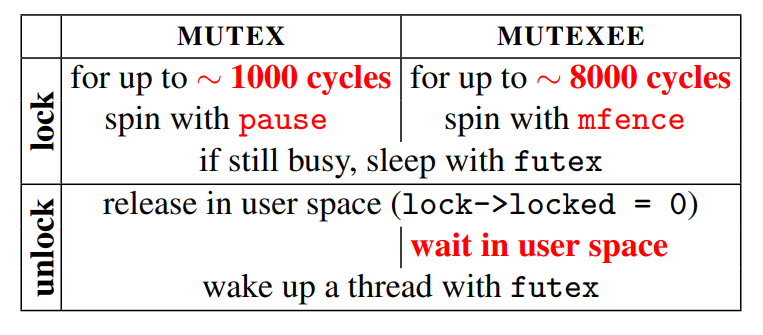
\includegraphics[scale=0.4]{images/img3.png}
\end{figure}

% 4.2.4
\subsubsection{表现}

由于公平性更差,Mutexee 的吞吐量能够达到 Mutex 的2.5 倍,但是有非常高的尾时延。如果通过设置自我唤醒时间来保证线程不会长时间睡眠,吞吐量又会打折扣。

% 4.3
\subsection{Proto}

% 4.3.1
\subsubsection{概述}

维护一个形式上的 MCS 队列,线程放锁后在进行锁的传递时,会跳过已进入睡眠的线程,将锁传递给它后继的第一个活跃的线程,跳过的线程组成一个链表,头节点在下一个执行临界区线程的节点中留存一份引用。

% 4.3.2
\subsubsection{具体策略}
\begin{enumerate}
    \item 线程拿锁时,简单使用 MCS 的方式进入队尾;
    \item 等待的线程有等待时间片,一段时间后会自动进入睡眠;
    \item 线程放锁时,向后遍历链表,如遇到睡眠线程则跳过,找到第一个活跃线程,将锁的所有权传给它,并在这个线程中留存一份跳过的线程组成的链表的头节点的引用,这个线程与跳过的线程组成一个循环链表;
    \item 当放锁后向后遍历找不到活跃的线程时,则唤醒睡眠的线程,继续进行锁的传递;
\end{enumerate}

\begin{figure}[ht]
    \centering
    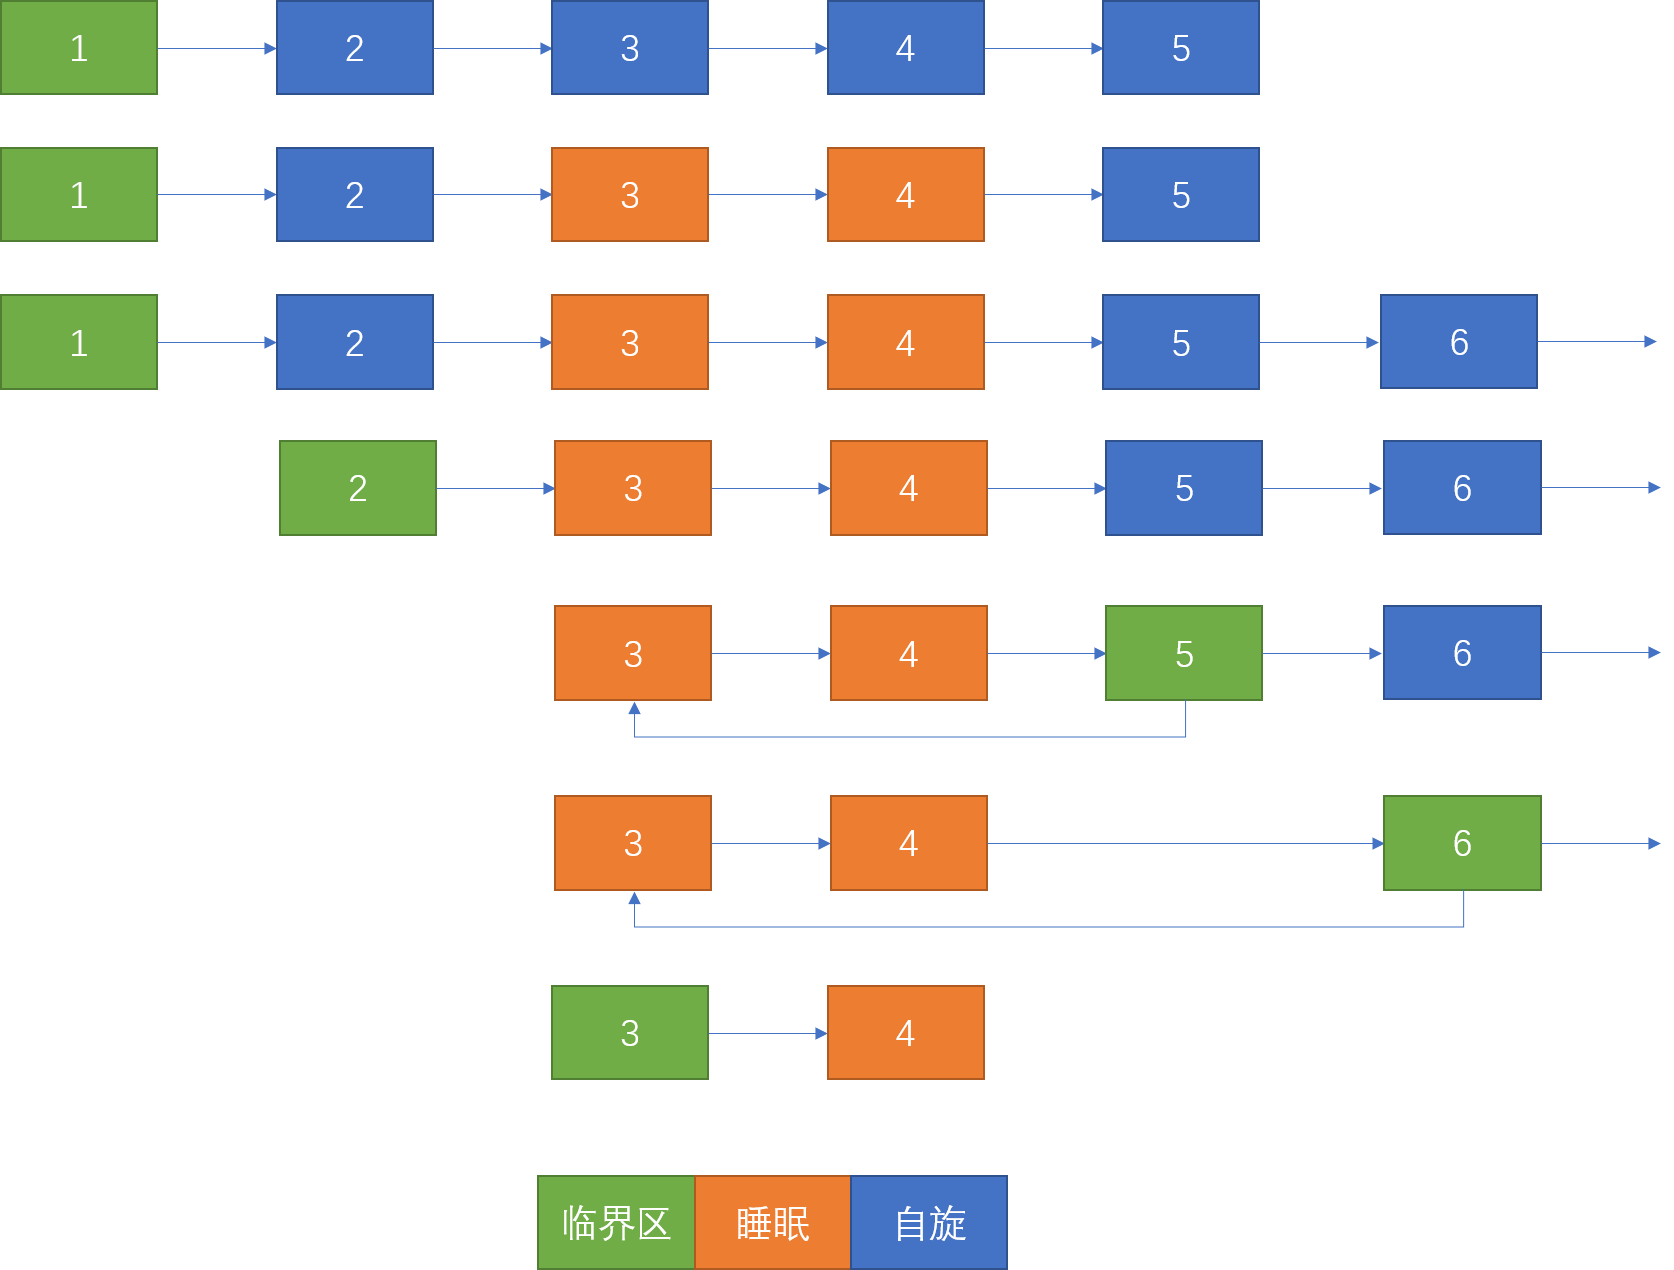
\includegraphics[scale=0.5]{images/img5.png}
\end{figure}

% 4.3.3
\subsection{表现}

\begin{enumerate}
    \item 通过在执行临界区的线程节点中存两个链表的引用,实现了逻辑上的单链表,事实上的双队列;
    \item 线程放锁时跳过睡眠线程,可以使活跃状态的线程尽快拿到锁以执行临界区,可以提高吞吐率;
    \item 进入睡眠的线程只有当活跃线程全部执行完后才能被唤醒,失去了部分公平性;
    \item 在放锁时需要遍历链表,在关键路径上引入额外开销;
\end{enumerate}

% 5
\section{对三种策略的数据分析}

在 8 核心的 Intel CPU 上,分别改变临界区长度与线程个数,对 pthread、Mutexee、MCS 策略进行对照实验。

统计在线程数量分别为16、32、48、64,临界区长度分别为8、16...64,以及64、128...1024的条件下,pthread、MCS、MutexEE三种策略的时延与吞吐率。

% 5.1
\subsection{16 线程下各指标随临界区长度(短)变化}

临界区长度为 8、16...64,属于短临界区,对比 Delay 为 200 与 100 时各指标的变化。Delay 为线程 routine 中循环内非临界区代码的长度。

\begin{enumerate}
    \item Delay 设为 200

    \begin{figure}[!h]
        \centering
        \begin{minipage}{0.49\linewidth}
            \centering
            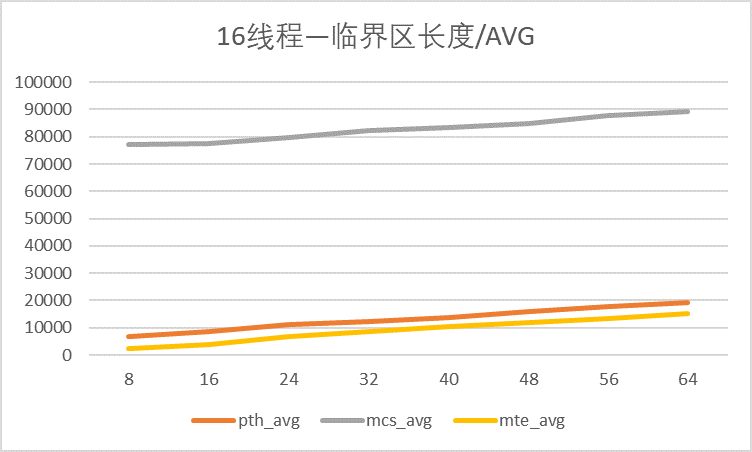
\includegraphics[scale=0.64]{../images/1.png}
        \end{minipage}
        \begin{minipage}{0.49\linewidth}
            \centering
            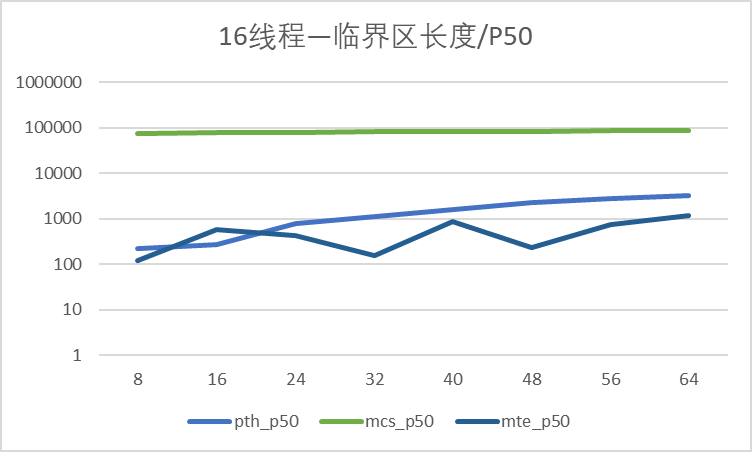
\includegraphics[scale=0.64]{../images/2.png}
        \end{minipage}
    \end{figure}

    \begin{figure}[!h]
        \centering
        \begin{minipage}{0.49\linewidth}
            \centering
            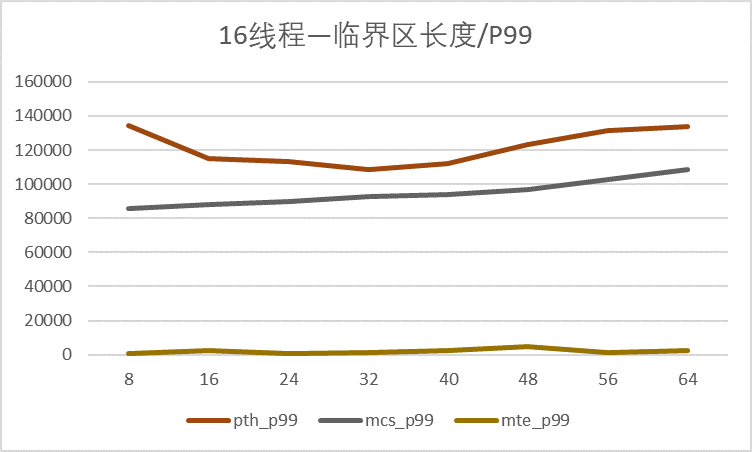
\includegraphics[scale=0.64]{../images/3.png}
        \end{minipage}
        \begin{minipage}{0.49\linewidth}
            \centering
            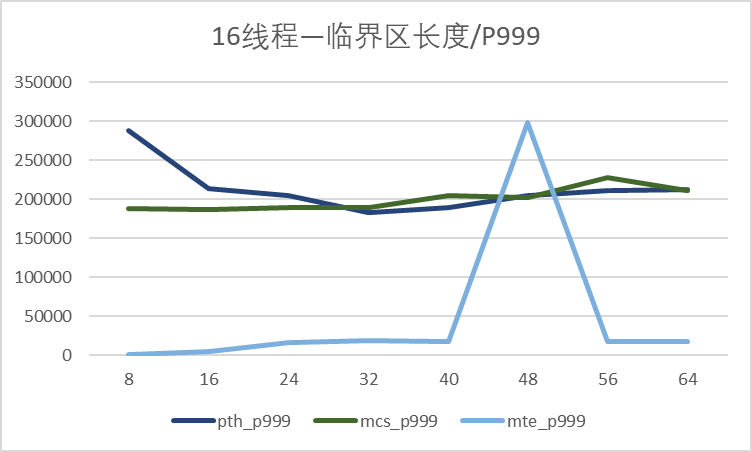
\includegraphics[scale=0.64]{../images/4.png}
        \end{minipage}
    \end{figure}

    \begin{figure}[!h]
        \centering
        \begin{minipage}{0.49\linewidth}
            \centering
            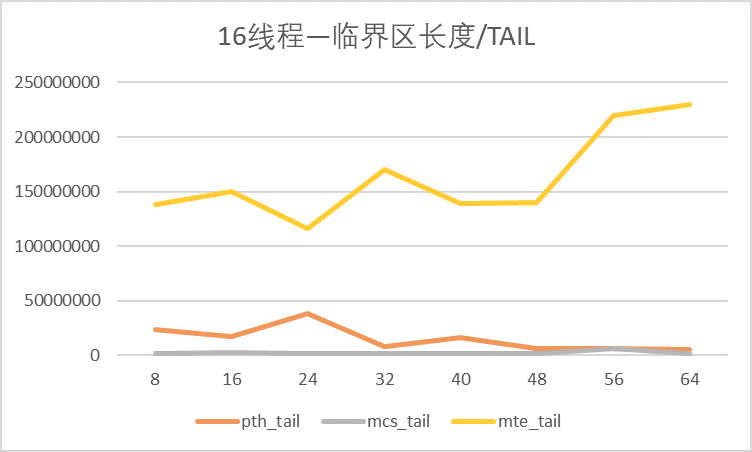
\includegraphics[scale=0.64]{../images/5.png}
        \end{minipage}
        \begin{minipage}{0.49\linewidth}
            \centering
            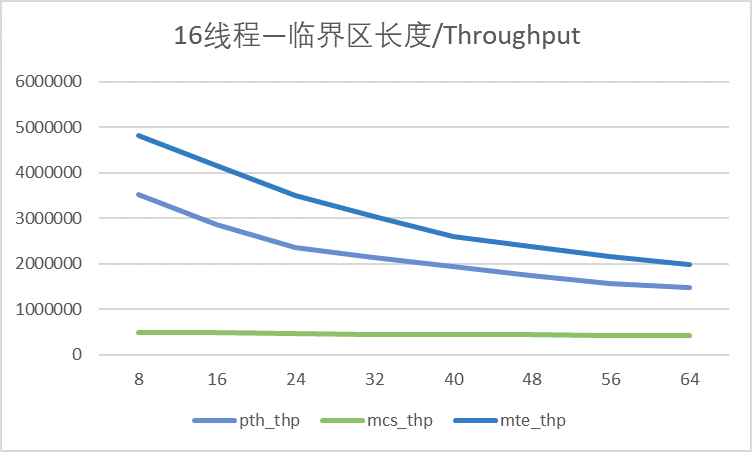
\includegraphics[scale=0.64]{../images/6.png}
        \end{minipage}
    \end{figure}

    \begin{itemize}
        \item 显然,对任意一种策略,随临界区长度增加,平均时延呈上升趋势,吞吐量呈下降趋势;
        \item 由于 Mutexee 的特性,存在大量入睡前等待的线程拿到了锁而导致少量已经入睡的线程一直拿不到锁,因此它的尾时延非常的高;并且,Mutexee 在临界区长为 48 时,P999 指标出现了意外的峰值,说明在这份 Mutexee 策略的实现所采用的入睡前与放锁后等待周期数,与CPU核心数,出现了类似共振的效应,使“尾时延”的比例扩展到了 P999;但是在线程数升到 64 后,P999 又降了下来,说明MutexEE策略下饥饿现象出现的概率随临界区长度的变化函数并非单调的,在临界区长为 48 时出现了极值;
        \item MCS 的平均时延远大于 pthread 与 Mutexee,吞吐量最低,但是尾时延非常小,主要原因在于 MCS 是公平的,在保证不存在饥饿(尾时延不高)的情况下,平均时延和吞吐量都不优秀;
        \item 在短临界区的情形下,Mutexee 确实比 pthread 实现了更低的平均时延与更高的吞吐量,得益于它的设计特性;但是 Mutexee 的尾时延非常高,因为它更容易导致饥饿;
        \item pthread 与 Mutexee 两种都是无法确保公平性的策略,Mutexee 为了降低平均延迟对饥饿的容忍度比 pthread 更高,也就是更为激进,因此它们各百分比的时延随临界区的变化趋势都不太稳定;而 MCS 因为保证了公平性,指标随临界区变化而上升或下降一直是严格的;
    \end{itemize}

    \item Delay 设为 100

    \begin{figure}[!h]
        \centering
        \begin{minipage}{0.49\linewidth}
            \centering
            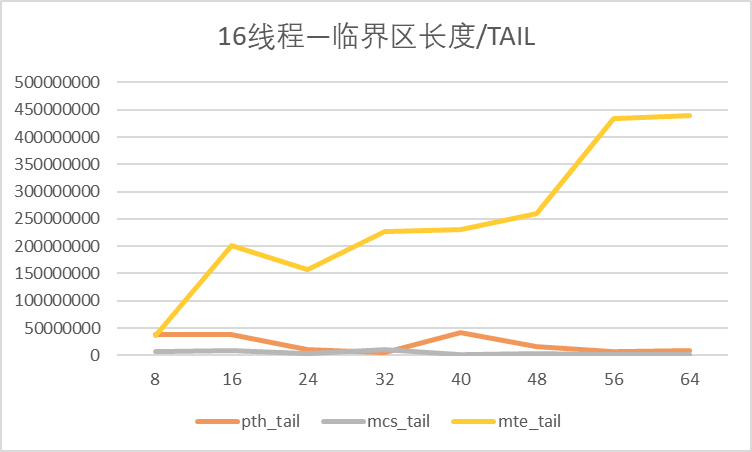
\includegraphics[scale=0.64]{../images/7.png}
        \end{minipage}
        \begin{minipage}{0.49\linewidth}
            \centering
            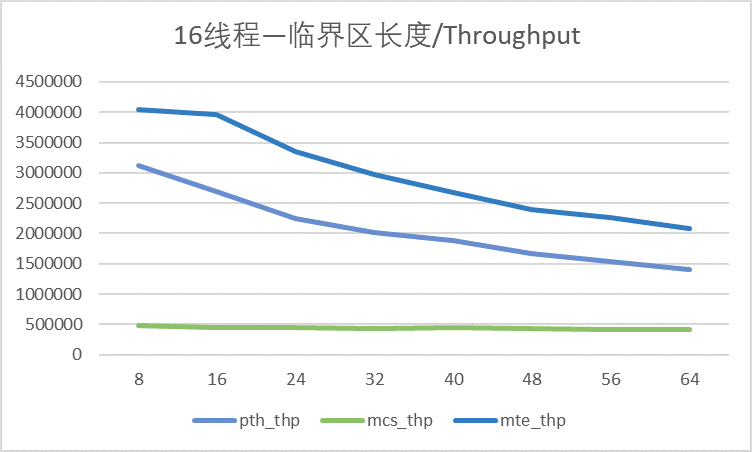
\includegraphics[scale=0.64]{../images/8.png}
        \end{minipage}
    \end{figure}

    \begin{itemize}
        \item 在 Delay 100 情形下,由于线程的竞争状态更为激烈,因此各策略的吞吐量相比 Delay 200 整体下降;
        \item 在 Delay 100 情形下,Mutexee 的尾时延在临界区上升时变化得更剧烈,说明竞争状态越强 Mutexee 出现饥饿现象的概率增幅越大;
    \end{itemize}

\end{enumerate}

% 5.2
\subsection{8 临界区长度下各指标随线程数变化}

线程数量为 8、16、24、32,由于 CPU 核心数为 8,在后面三种情况下符合 Over Subscription。Delay 设为 200。

\begin{figure}[!h]
    \centering
    \begin{minipage}{0.49\linewidth}
        \centering
        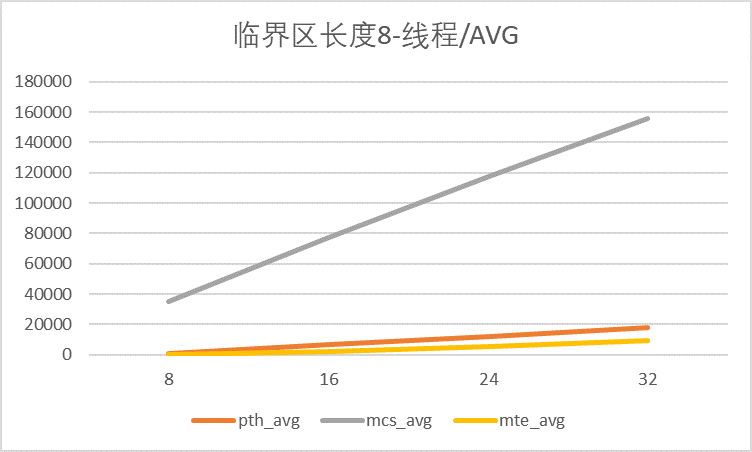
\includegraphics[scale=0.64]{../images/9.png}
    \end{minipage}
    \begin{minipage}{0.49\linewidth}
        \centering
        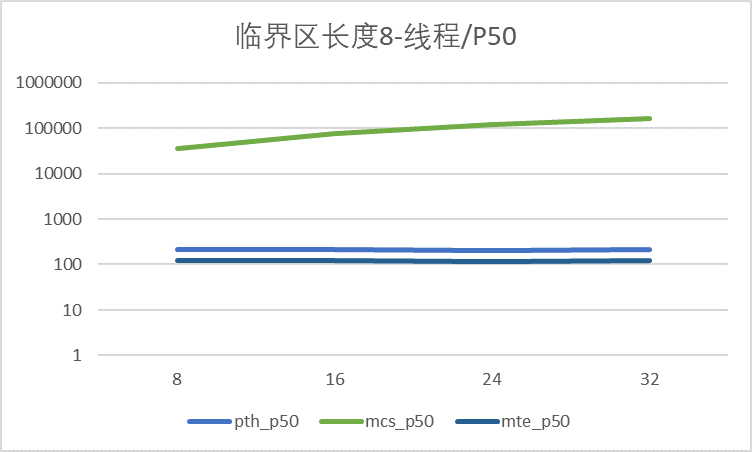
\includegraphics[scale=0.64]{../images/10.png}
    \end{minipage}
\end{figure}

\begin{figure}[!h]
    \centering
    \begin{minipage}{0.49\linewidth}
        \centering
        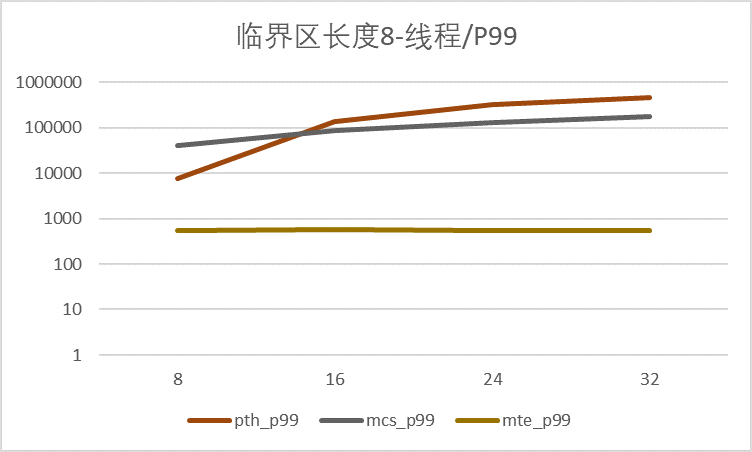
\includegraphics[scale=0.64]{../images/11.png}
    \end{minipage}
    \begin{minipage}{0.49\linewidth}
        \centering
        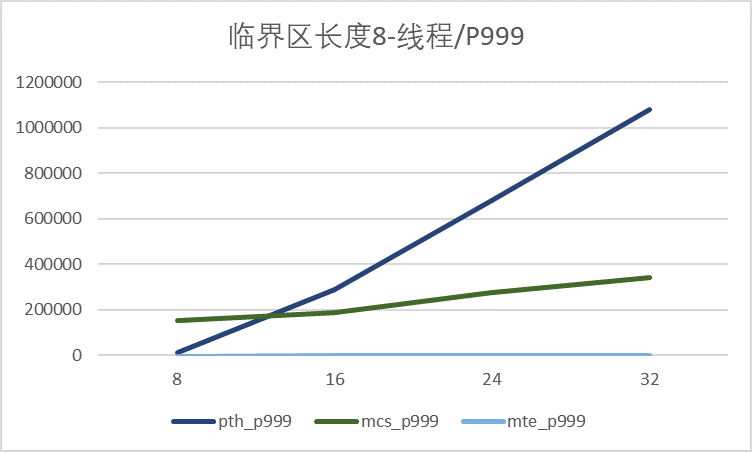
\includegraphics[scale=0.64]{../images/12.png}
    \end{minipage}
\end{figure}

\begin{figure}[!h]
    \centering
    \begin{minipage}{0.49\linewidth}
        \centering
        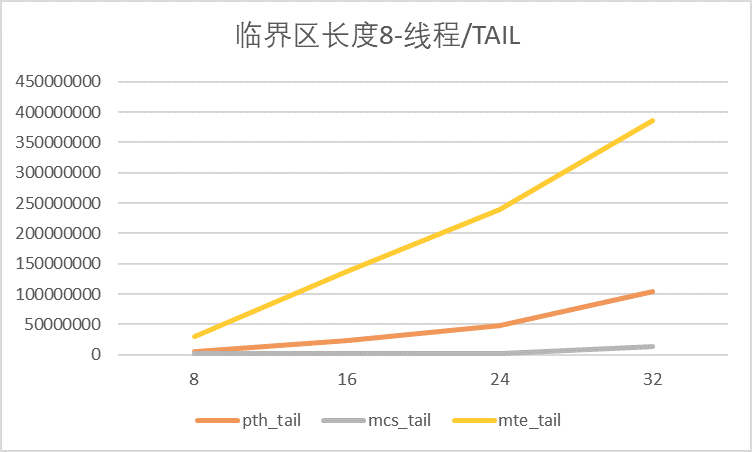
\includegraphics[scale=0.64]{../images/13.png}
    \end{minipage}
    \begin{minipage}{0.49\linewidth}
        \centering
        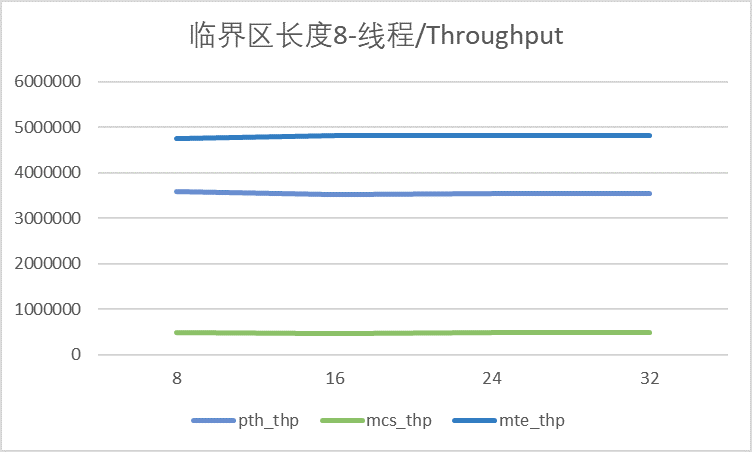
\includegraphics[scale=0.64]{../images/14.png}
    \end{minipage}
\end{figure}

\newpage

\begin{itemize}
    \item 临界区长度一定时,各指标随线程数量的变化,基本都趋于线性变化;

    \item 在没有出现 Over Subscription 现象时,线程数量较少,pthread 策略表限较好,但是线程数量增加后,pthread的时延(除了尾时延)比 MCS 和 Mutexee 上升得更快,尤其是 P99 与 P999,由于 Mutexee 擅长临界区较短的情况,pthread的时延(除了尾时延)都比 Mutexee 高;
\end{itemize}

\subsection{16 线程下各指标随临界区长度(长)变化}

临界区长度为 64、128...1024,属于长临界区。Delay 设为 200。

\begin{figure}[!h]
    \centering
    \begin{minipage}{0.49\linewidth}
        \centering
        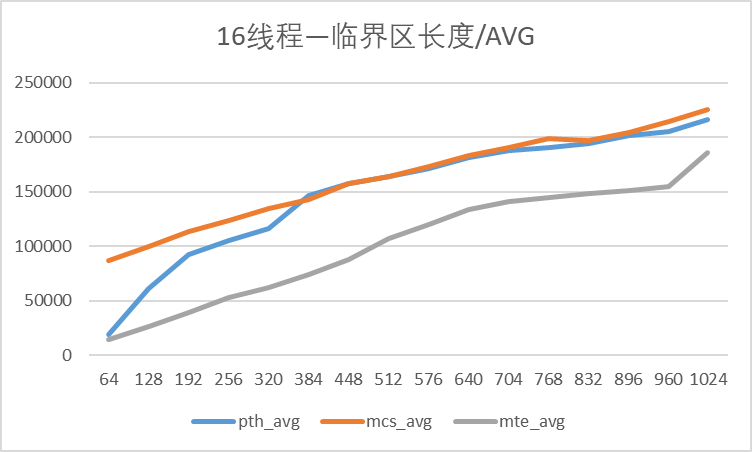
\includegraphics[scale=0.64]{../images/15.png}
    \end{minipage}
    \begin{minipage}{0.49\linewidth}
        \centering
        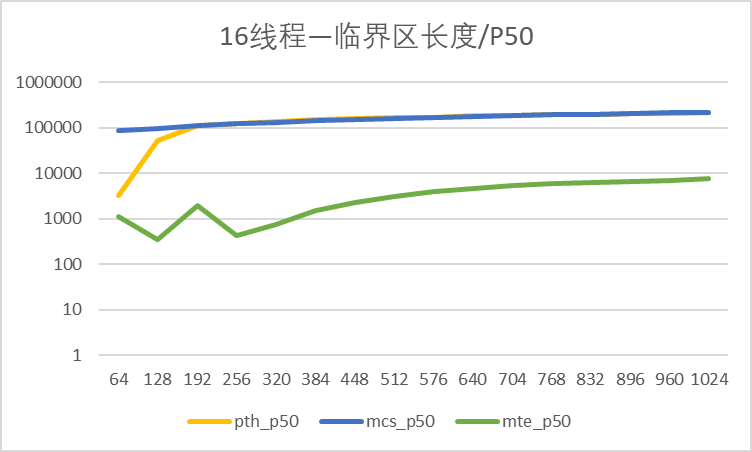
\includegraphics[scale=0.64]{../images/16.png}
    \end{minipage}
\end{figure}

\begin{figure}[!h]
    \centering
    \begin{minipage}{0.49\linewidth}
        \centering
        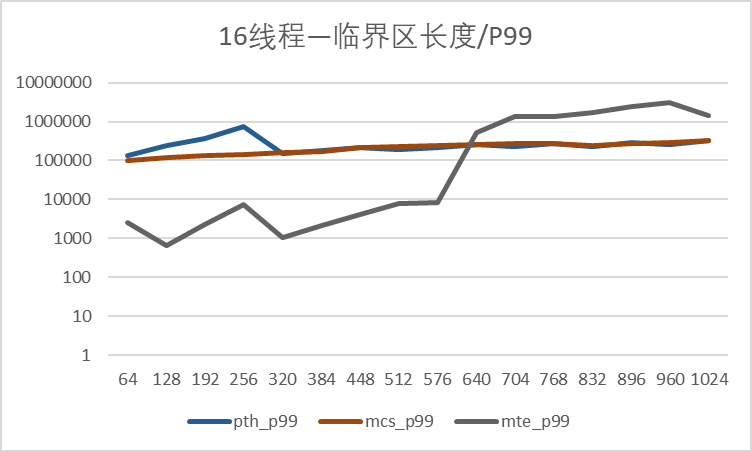
\includegraphics[scale=0.64]{../images/17.png}
    \end{minipage}
    \begin{minipage}{0.49\linewidth}
        \centering
        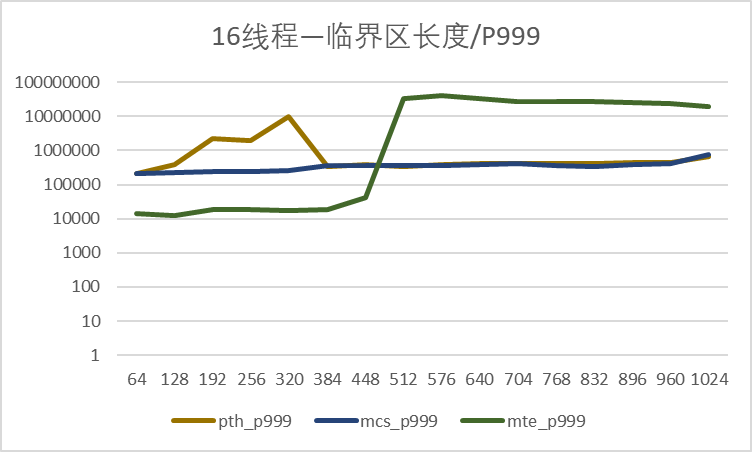
\includegraphics[scale=0.64]{../images/18.png}
    \end{minipage}
\end{figure}

\begin{figure}[!h]
    \centering
    \begin{minipage}{0.49\linewidth}
        \centering
        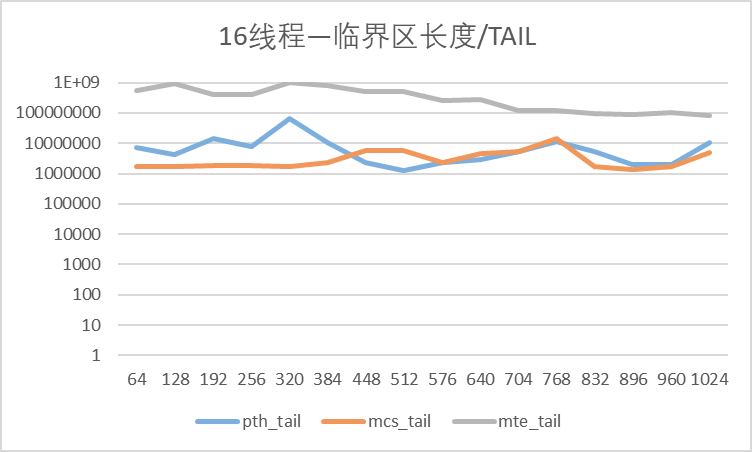
\includegraphics[scale=0.64]{../images/19.png}
    \end{minipage}
    \begin{minipage}{0.49\linewidth}
        \centering
        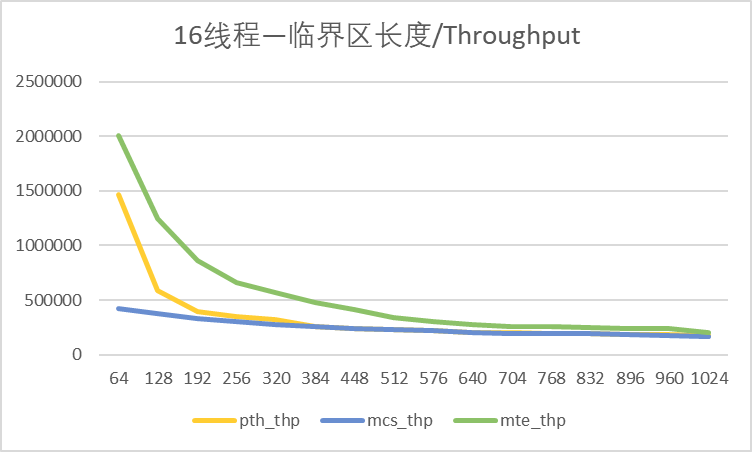
\includegraphics[scale=0.64]{../images/20.png}
    \end{minipage}
\end{figure}

\newpage

\begin{itemize}
    \item 在临界区长度较长时,pthread 与 MCS变得逐渐趋近——由于本身时间就长,线程数不多,pthread 导致的饥饿现象随临界区长度变长而变得不明显;
    \item 在临界区长度较长时,Mutexee 虽然能够保证平均时延比另外两种更低,但是其表现显然比如临界区短时优异了;
    \item Mutexee 的 P99 与 P999 在临界区长度变长时有个突然上升的过程,说明瓶颈已到,其尾时延比临界区较短时更为糟糕;
    \item 虽然 Mutexee 的等待循环数是可以更改的,但是无法动态适应场景,在本实验中只适用于短临界区;
\end{itemize}

% 6
\section{新策略的设计}

且将本策略命名为 ACE 调度策略。

% 6.1
\subsection{思路}

\begin{enumerate}
    \item MCS 锁是一种十分精巧的策略,但它与任何一种阻塞策略搭配,最后的结果都不那么令人满意;如果使用忙等,那么整个等待队列中所有线程都在忙等,但是后面的大量线程明显是没有必要处于自旋状态的,它们的忙等不仅浪费能量,还会抢占持有锁线程的资源;如果使用阻塞,那么前面的线程明明很快能获取锁却还要经历唤醒,产生没有必要的时延;本策略在综合分析MCS的特性之后提出,与 MCS 的思想非常类似;
    \item 策略原则为,每个核心上只存在一个处于活跃态的线程,其他线程全部阻塞。存在一个 MCS 主队列,主队列上排列的是所有活跃线程;对于一个核心,核心上的所有线程排成一个MCS队列,队头是当前核心上的活跃线程,其他为阻塞线程;
    \item 当有新的线程要获取锁,它首先通过原子操作使自己进入自己核心的队列,如果它是核心中的第一个线程,那么再通过原子操作使自己进入主队列,否则进入阻塞态;进入主队列后,如果它是主队列第一个线程,那么直接获取锁,否则进入自旋态;
    \item 线程被解除自旋态,到获取锁之前,它需要将自己核心队列的下一个线程唤醒,那么下一个线程就会自己进入主队列;
    \item 线程放锁时,将主队列的下一个线程解旋,那么下一个线程又唤醒自己核心的下一个线程...
\end{enumerate}

\newpage

% 6.2
\subsection{具体实现}

% 6.2.1
\subsubsection{数据结构}

\begin{itemize}
    \item 链表
    \item 各 CPU 核心队列尾节点指针数组
    \item 活跃队列尾节点指针
\end{itemize}

\begin{lstlisting}
struct QNode {
    int cpu_id;
    QNode *block_next;       // Successor node of same cpu
    QNode *active_next;      // Successor node of active queue
};

QNode *activeTail;           // Tail of active queue
QNode *coreTails[n];         // Array of tail of all cpus' queue
\end{lstlisting}

% 6.2.2
\subsubsection{线程拿锁}

\begin{lstlisting}
void lock(QNode *node) {
    // Enqueue locally
    QNode *org = getAndSet(&coreTails[node->cpu_id], node);
    if (org) {
        // There's an active thread of this cpu
        org->block_next = node;
        // Switch to block state
        sleep();
    }

    // Enqueue globally
    QNode *prev = getAndSet(&activeTail, node);
    if (prev) {
        // There's a thread working in critical section
        prev->activeNext = node;
        // Switch to spin state
        spin();
    }
    // Awake the successor of current cpu
    if (node->block_next) {
        awake(node->block_next);
    }
}
\end{lstlisting}

\newpage

% 2.3.3
\subsubsection{线程放锁}

\begin{lstlisting}
void unlock(QNode *node) {
    if (node->active_next) {
        despin(node->active_next);
    }
    // May need to free the node's memory
}
\end{lstlisting}

% 2.3.4
\subsubsection{分析}

\begin{itemize}
    \item 本策略本质上是一个双层的 MCS 队列,主队列是 MCS 队列,每个核心自己的队列也是 MCS 队列;
    \item 本策略将传统 MCS 对线程严格维护先来后到的原则,改变为对每个核心维护先来后到的原则,每个核心内部的线程也维护先来后到的原则,因此也满足相对公平;
    \item 本策略折衷解决了 MCS 不能适应单纯地适应 spin 与 spin-then-park 策略的问题,将后面的线程被唤醒的时延分散到了同核心的活跃线程拿锁时,使这部分时延不至于暴露在关键路径上,理论上能够提高 Over Subscription 情况下的吞吐量;
\end{itemize}

\end{document}
